\documentclass{sigchi}

% Use this section to set the ACM copyright statement (e.g. for
% preprints).  Consult the conference website for the camera-ready
% copyright statement.

% Copyright
\CopyrightYear{2020}
%\setcopyright{acmcopyright}
\setcopyright{acmlicensed}
%\setcopyright{rightsretained}
%\setcopyright{usgov}
%\setcopyright{usgovmixed}
%\setcopyright{cagov}
%\setcopyright{cagovmixed}
% DOI
\doi{https://doi.org/10.1145/3313831.XXXXXXX}
% ISBN
\isbn{978-1-4503-6708-0/20/04}
%Conference
\conferenceinfo{CHI'20,}{April  25--30, 2020, Honolulu, HI, USA}
%Price
\acmPrice{\$15.00}

% Use this command to override the default ACM copyright statement
% (e.g. for preprints).  Consult the conference website for the
% camera-ready copyright statement.

%% HOW TO OVERRIDE THE DEFAULT COPYRIGHT STRIP --
%% Please note you need to make sure the copy for your specific
%% license is used here!
% \toappear{
% Permission to make digital or hard copies of all or part of this work
% for personal or classroom use is granted without fee provided that
% copies are not made or distributed for profit or commercial advantage
% and that copies bear this notice and the full citation on the first
% page. Copyrights for components of this work owned by others than ACM
% must be honored. Abstracting with credit is permitted. To copy
% otherwise, or republish, to post on servers or to redistribute to
% lists, requires prior specific permission and/or a fee. Request
% permissions from \href{mailto:Permissions@acm.org}{Permissions@acm.org}. \\
% \emph{CHI '16},  May 07--12, 2016, San Jose, CA, USA \\
% ACM xxx-x-xxxx-xxxx-x/xx/xx\ldots \$15.00 \\
% DOI: \url{http://dx.doi.org/xx.xxxx/xxxxxxx.xxxxxxx}
% }

% Arabic page numbers for submission.  Remove this line to eliminate
% page numbers for the camera ready copy
% \pagenumbering{arabic}

% Load basic packages
\usepackage{balance}       % to better equalize the last page
\usepackage{graphics}      % for EPS, load graphicx instead 
\usepackage[T1]{fontenc}   % for umlauts and other diaeresis
\usepackage{txfonts}
\usepackage{mathptmx}
\usepackage[pdflang={en-US},pdftex]{hyperref}
\usepackage{color}
\usepackage{booktabs}
\usepackage{textcomp}
\usepackage{graphicx}

% Some optional stuff you might like/need.
\usepackage{microtype}        % Improved Tracking and Kerning
% \usepackage[all]{hypcap}    % Fixes bug in hyperref caption linking
\usepackage{ccicons}          % Cite your images correctly!
% \usepackage[utf8]{inputenc} % for a UTF8 editor only

% If you want to use todo notes, marginpars etc. during creation of
% your draft document, you have to enable the "chi_draft" option for
% the document class. To do this, change the very first line to:
% "\documentclass[chi_draft]{sigchi}". You can then place todo notes
% by using the "\todo{...}"  command. Make sure to disable the draft
% option again before submitting your final document.
\usepackage{todonotes}

% Paper metadata (use plain text, for PDF inclusion and later
% re-using, if desired).  Use \emtpyauthor when submitting for review
% so you remain anonymous.
\def\plaintitle{CSCM69: Human-Centred Perspectives and Methods\\Coursework 2 - Work/Life Balence}
\def\plainauthor{Andy Gray}
\def\emptyauthor{}
\def\plainkeywords{Authors' choice; of terms; separated; by
  semicolons; include commas, within terms only; this section is required.}
\def\plaingeneralterms{Documentation, Standardization}

% llt: Define a global style for URLs, rather that the default one
\makeatletter
\def\url@leostyle{%
  \@ifundefined{selectfont}{
    \def\UrlFont{\sf}
  }{
    \def\UrlFont{\small\bf\ttfamily}
  }}
\makeatother
\urlstyle{leo}

% To make various LaTeX processors do the right thing with page size.
\def\pprw{8.5in}
\def\pprh{11in}
\special{papersize=\pprw,\pprh}
\setlength{\paperwidth}{\pprw}
\setlength{\paperheight}{\pprh}
\setlength{\pdfpagewidth}{\pprw}
\setlength{\pdfpageheight}{\pprh}

% Make sure hyperref comes last of your loaded packages, to give it a
% fighting chance of not being over-written, since its job is to
% redefine many LaTeX commands.
\definecolor{linkColor}{RGB}{6,125,233}
\hypersetup{%
  pdftitle={\plaintitle},
% Use \plainauthor for final version.
%  pdfauthor={\plainauthor},
  pdfauthor={\emptyauthor},
  pdfkeywords={\plainkeywords},
  pdfdisplaydoctitle=true, % For Accessibility
  bookmarksnumbered,
  pdfstartview={FitH},
  colorlinks,
  citecolor=black,
  filecolor=black,
  linkcolor=black,
  urlcolor=linkColor,
  breaklinks=true,
  hypertexnames=false}

% create a shortcut to typeset table headings
% \newcommand\tabhead[1]{\small\textbf{#1}}

% End of preamble. Here it comes the document.
\begin{document}

\title{\plaintitle}

\numberofauthors{1}
\author{%
  \alignauthor{??\\
    \affaddr{??}\\
    \affaddr{Swansea, Wales}\\
    \email{??@swansea.ac.uk}}
}
\maketitle

\begin{abstract}
	one one one one one one one one one one one one one one one one one one one one one one one one one one one one one one one one one one one one one one one one one one one one one one one one one one one one one one one one one one one one one one one one one one one one one one one one one one one one one one one one one one one one one one one one one one one one one one one one one one one one one one one one one one one one one one one one one one one one one one one one one one one one one one one one one one one one one one one one one one one one one one one one one one one one one one 
	
\end{abstract}


% ACM Classfication

\begin{CCSXML}
<ccs2012>
<concept>
<concept_id>10003120.10003121</concept_id>
<concept_desc>Human-centered computing~Human computer interaction (HCI)</concept_desc>
<concept_significance>500</concept_significance>
</concept>
<concept>
<concept_id>10003120.10003121.10003125.10011752</concept_id>
<concept_desc>Human-centered computing~Haptic devices</concept_desc>
<concept_significance>300</concept_significance>
</concept>
<concept>
<concept_id>10003120.10003121.10003122.10003334</concept_id>
<concept_desc>Human-centered computing~User studies</concept_desc>
<concept_significance>100</concept_significance>
</concept>
</ccs2012>
\end{CCSXML}

\ccsdesc[500]{Human-centered computing~Human computer interaction (HCI)}
\ccsdesc[300]{Human-centered computing~Haptic devices}
\ccsdesc[100]{Human-centered computing~User studies}

% Author Keywords
\keywords{\plainkeywords}

% Print the classficiation codes
\printccsdesc
Please use the 2012 Classifiers and see this link to embed them in the text: \url{https://dl.acm.org/ccs/ccs_flat.cfm}



\section{Introduction}
	Harvard conducted a survey which asked professional people how many hours they worked a week, 94\% said they put in more than 50 hours or more. Out of these professionals, 50\% said they are working 65 or more hours \cite{harvard_review}. What is even more staggering is that this survey got done in 2009, a time where Blackberry mobile phones were all the rage and iPhones had only been on the market for around two years. This year was when the iPhone 3G was just about to hit stores and was way before the iPhone 4 and where the smartphone, as we currently know them, indeed took off and changed the way we interact with our mobile devices. As the Harvard survey also found out that 20-25 hours a week get spent monitoring their Blackberrys while outside of working hours \cite{harvard_review}. 
	
	
	These numbers show that a work-life balance has been an issue for some years. Especially when looking at statistics published in 2020, by the NY Post's Business Insider, that state 48\% of Americans consider themselves workaholics and the CNBC stating that 66\% of American works lacking a healthy work-life balance \cite{work-life_2020}. A staggering fact that we can relate to from experience is that 77\% of full-time works suffer from burnout from their current job \cite{work-life_2020}. Rescue Time analysed their users' data in 2019 and found that 40\% of people used their computers after 10 pm and 28\% of people start their workday before 8:30 am \cite{rescuetime_study}.  
	
	What we aim to do within this report is to identify some of the leading apps that get associated with work-life balance. Once these apps get identified, we aim to investigate these tools while critiquing their designs concerning their interactions with HCI. These apps include \textbf{[list apps here]}, we will then be interviewing users and finding out their views on these applications and how they have impacted their work-life balance.
	
	%[Overview of the assignment]
	  

\section{Existing apps and devices used Widley in Work-Life Balance}
	% Find out what key existing apps, services and devices are widely used in the domain of interest that you have chosen. For example, this might include fitness trackers, creativity support apps or other domain-specific services. As a guide, I would expect you to find around 3–5 tools here.
	
	"With the pervasiveness of technology, it has not only permeated our workspaces but it has also become invasive in our private personal spaces \cite{peters2012sig}." This quote got taken from a CHI paper published in 2012. In this paper, they state what defines a work-life balance is on the worker working longer than 50 hours a week compared to personal care and leisure whether it gets paid, or unpaid, but for women that also include the rate of employees who have children \cite{peters2012sig}. With this definition in mind, we are going to identify and critique four apps and devices that have made an impact for good and bad reasons for people's work-life balance. The applications and devices we will be looking at are emails, instant messaging (IM), meditation apps and mobile phone devices.
	
	%Email
	One application that has brought about both good things and bad things for work-life balance is the email. While it made communication more accessible, especially in the early days as we did not have to wait for a letter to get sent in the post, it has now become very consuming. In result, it has created a sense of urgency around reading and responding to emails straight away \cite{stawarz2013d}. However, in terms of work, email has improved the efficiency of working when aiming to communicate with colleges or other people when they are not physically present.
	
	%IM
	An application that has both a positive and negative effect on work-life balance is instant messaging, for example, WhatsApp, iMessage, Facebook Message, Slack. IM has shown how the same communication channel often gets used personal activities and work arrangements. In some cases, both personal and work activities get almost done at the same time \cite{lindley2012s}. However, IM has become an alternative method to the traditional communication methods for both work \cite{siggroup2005group} and private communication \cite{flanagin2005online}, instead of it being an additional medium on top. However, IM, by its very definition, is an interruption, especially if we use the definition defined by O'Conaill \& Frohlich, "a synchronous interaction which is not initiated by the recipient, is unscheduled, and results in the recipient discontinuing their current activity" \cite{rennecker2003theorizing}. 
	
	%Meditation Apps
	In the hustle and bustle of the modern-day life, especially while at the time of writing being in a second national lockdown in the UK and a global pandemic happening, public's perception around mental health has started to shift focus. Applications that get promoted to help with mental health and lockdown are meditation apps. While mindful apps do help with well being and mental health, however, they require training in order to be completely effective \cite{dauden2018evaluating}.  Mindfulness gets defined as the "awareness that arises through paying attention on purpose, in the present moment without judgment \cite{baer2003mindfulness}". A study of mindful applications has found that only 4\% provide any form of mindfulness training, the rest only offer time reminders for doing meditation \cite{mani2015review}. 
	
	%Mobile
	The one technology that has made both work-life better and worse at the same time, depending on what angle it gets looked at is the mobile phone. Through the introduction of mobile phones, it has made it very difficult to separate work-life \cite{gronvall2016hci, sadler2006balancing} as all the previous apps have demonstrated. This issue is a result of the mobile phone being the one device that enables all of these. Mobile phones have created a grey area between private and work domains, which is why much research is getting carried out in this area \cite{fleck2015balancing}. As studies have shown that Workers average just 2 hours and 48 minutes of productive device time a day and check emails and IM about every 6 minutes on average \cite{rescuetime_study}. We wonder if this is a result of mobile phones and them being so available and accessible to "just check" at any points.
	
	\section{Critiquing Existing Apps and Devices for Work-Life Balance}
	
	We will now be critiquing existing apps and devices within the areas that we have identified as widely used within the work-life balance. We will be identifying one app or device, within the different areas, and then critiquing them, aiming to identify how they could be adapted to amplify the user's experience. We will be looking at how the app or device makes it a particular part of being human, and how they aim to do this and possibly how they could do it better.
	
		\subsection{Mobile Device)}
		% Critique the device
		% Have work/life modes - like light or dark mode.
		Mobile devices have been around for many years until the introduction of the smartphone, that we know today, laptops were the only primary way to do any form of real work on the go. However, these did have their limitations and their pros. However, since the introduction of smartphones, and how powerful and capable they now are, mobile devices and the ability to do work from them has increased and become more proficient. While there are many smartphone devices out there, we will be focusing on Apple's iPhone for our critique. We have chosen this device primarily due to our more familiarity with the device and what it can do. 
		
		The mobile device, in the modern-day, is an essential item for most people. People use them for a while range of things, whether it be for socialising, relaxing by play games, for example, or get used for business. No one device has given the user so much freedom in what it can allow to user to do before, while still be relatively small and can be carried in just a pocket. However, the applications and features that enable us to do so much. They can and do get used for so much more than what its intention was. For example, social media intended to connect people around the world if we take Facebook in this case. However, it has now not only become a platform to allow people to communicate, but it has allowed the business to have a platform to be able to trade from that would not have been their before. So social media is also business media, or is still social media? As we can see, a vast grey area has got generated, which we believe through mobile phones to how accessible they are and how they connect to the internet 24/7 unless the user has run out of data allowance, and world wide web. However, this ability to have so much content on-demand, we could say, has created a form of addiction but this could be down to their interruption nature, through notifications and attention-grabbing features like ringtones, and haptic vibrates. So with mobile phones getting used for social and work, is there any surprise that works are not super productive within a typical workday or struggle to switch off from work. While we have used social media as an example, in this case, it is valid for several different applications available, like emails, instant messaging and socialising. We believe as they are all in one place, it has made it harder to maintain an excellent work-life balance.
		
		A feature that we believe would genuinely enhance the user's experience and help with the work-life balance is to have an option that will allow the mobile device to flip between work and personal modes. What this feature would allow the user to do is list applications on their mobile device that are work-related, and then list all the apps that are personal life-related. The user will then be able to designate a time of where they should be at work and not, which then activates the app lists on either one to operate. For example, if it is not in work time, then all the work-related apps will be deactivated with no notifications appearing, and if the user tries to log into one of these apps, then a message will appear saying it is not in the working hours. Also, within work time, all the personal apps that are likely to create distractions are deactivated, and the same thing then happens to them. We believe this feature would, by having physical restrictions, make the users more aware of what they are doing and then be more mindful about their work-life balance. Therefore, as a result, enhancing both their work lives and their personal lives.
		
		\subsection{Email}
		% Critique the app
		Emails when they got first created brought about significant changes within the communication area. An email allowed a user to be able to send a document to another user instantly meaning that no longer do people have to wait for a document to be snd in the post and delivered if there were no fax machines available. However, emails have now evolved from business use to now a mixture of both. A single user is now likely to be having multiple accounts, private and work, with the user not only receiving potential vital documents like car insurance documents, for example, they could also be receiving advertisements in emails from companies.
		
		With users now having multiple email address email applications, like Apple's mail, allows the user to attach multiple email address to the app to all get viewed within the application. While this is a great feature and truly puts the user at the centre of allowing them to view all their different possible emails in one place, instead of logging into multiple email provider application. However, it has also created a significant overlap of what is work and work is life. We believe this is a result of the application trying to be helpful and provide the user with all their emails. However, what it fails to do is to distinguish the difference between work and private email addresses and notifies the user when an email comes through, work or personal. Which we believe adds to the anxiety of emails and the need to have to respond instantly.  We believe that a great feature would be to be able to distinguish which address is work and which ones are private and then create an automatic out of office style notification to the sender but does not display to the user until their designated work time.
		
		\subsection{Mindful Application - Calm}
			% https://usabilitygeek.com/ux-case-study-calm-mobile-app/
		
		\subsection{Instant Messaging}
		IM is an application that genuinely changed the way people communicated. Instead of everything seeming very formal in the way of an email, and without having the limitations of using mobile text message, whether its a lack of available credit or limited character limits, IM allowed users to be able to communicate more naturally over the internet for free. With the responses being almost instant, depending on the user's internet speed. Our first experience of this was with Microsoft Network (MSN) in the mid-2000s. This service truly put the user first and allowed users, as long as they were both logged on, communicate with each other. To top it all off, it was all for free. However, this started to take on a new direction when mobile phones started to become very popular and capable. Traditional text messages more moved into IM, and critical apps like WhatsApp started to emerge. This app was great as it allowed users, regardless of the operating system of their device used, to communicate with each other for free. Also, users were able to send images to each other without incurring a network fee.
		
		Even though apps like WhatApp has brought about some actual benefits, it has also blurred the lines of work-life balance. With the messages and IM being distractive by nature, affecting workflow and work colleges contacting people using these services but out of work time. On top of that, a feature allows people within WhatsApp to see if the sender to see if the recipient of the message has read the message, but in the relation of work relationships, this could cause frustration and add to the sense of anxiety to communicate straight away not to upset someone especially if it is the user's boss thats sending the message. The app will show the sender that the user has read the message but not responded, even if it is not in working hours. Therefore, having an impact on work-life balance and boundaries.
		
		While WhatsApp has brought about tremendous benefits, WhatsApp puts all the user's conversations, whether it be personal all or work-related all within once place. With the work-life divide becoming much unclearer, a great feature would be to allow the user to label contacts as personal or work-related. With the contacts being label then, the application can then group the contacts or conversations as appropriate.  Additionally, the application could then stop any work messages getting sent or seen out of work hours and any non-work messages getting shown in work hours. However, if a message needs to get sent urgently a command likes Apple's driving mode setting on iPhones, sending urgent, could be used to get the message sent out of the allocated time.
	

%\begin{figure}
%	\begin{center}
%		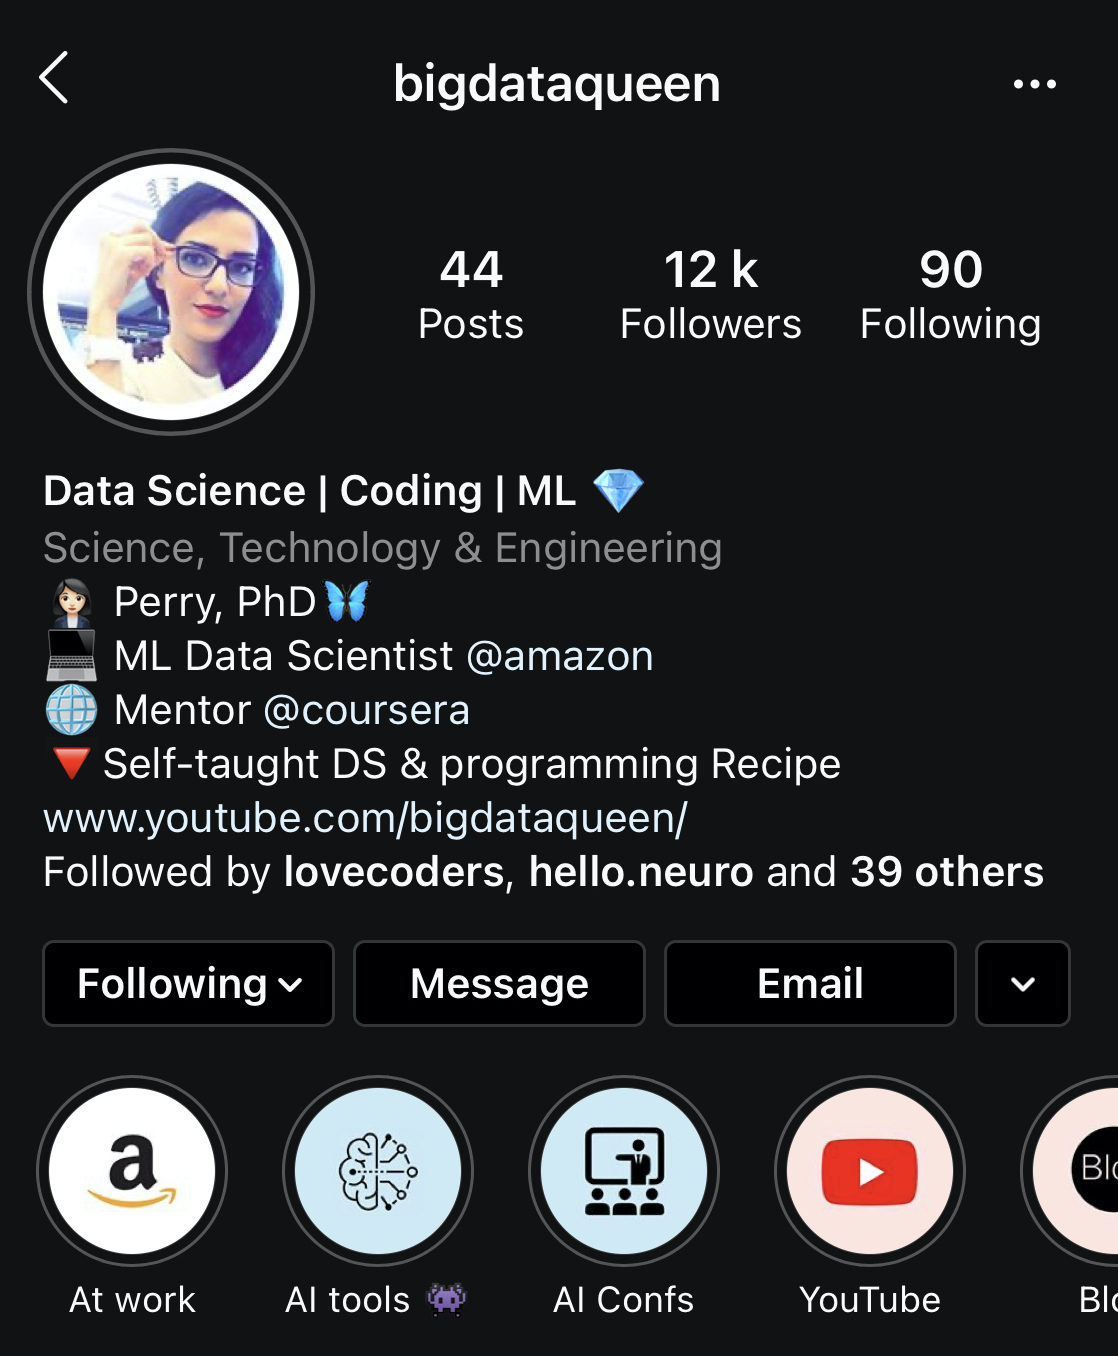
\includegraphics[width=5cm]{instagram_example2.jpeg}
%		\caption{An Instragram user profile overview. This is @bigdataqueen public profile overview.}
%		\label{fig:instagram_overview}
%	\end{center}
%\end{figure}


\section{Design an User Study? -> That what its called?}
	explain what will be included int he US and why made choices?

%\begin{figure}
%	\begin{center}
%		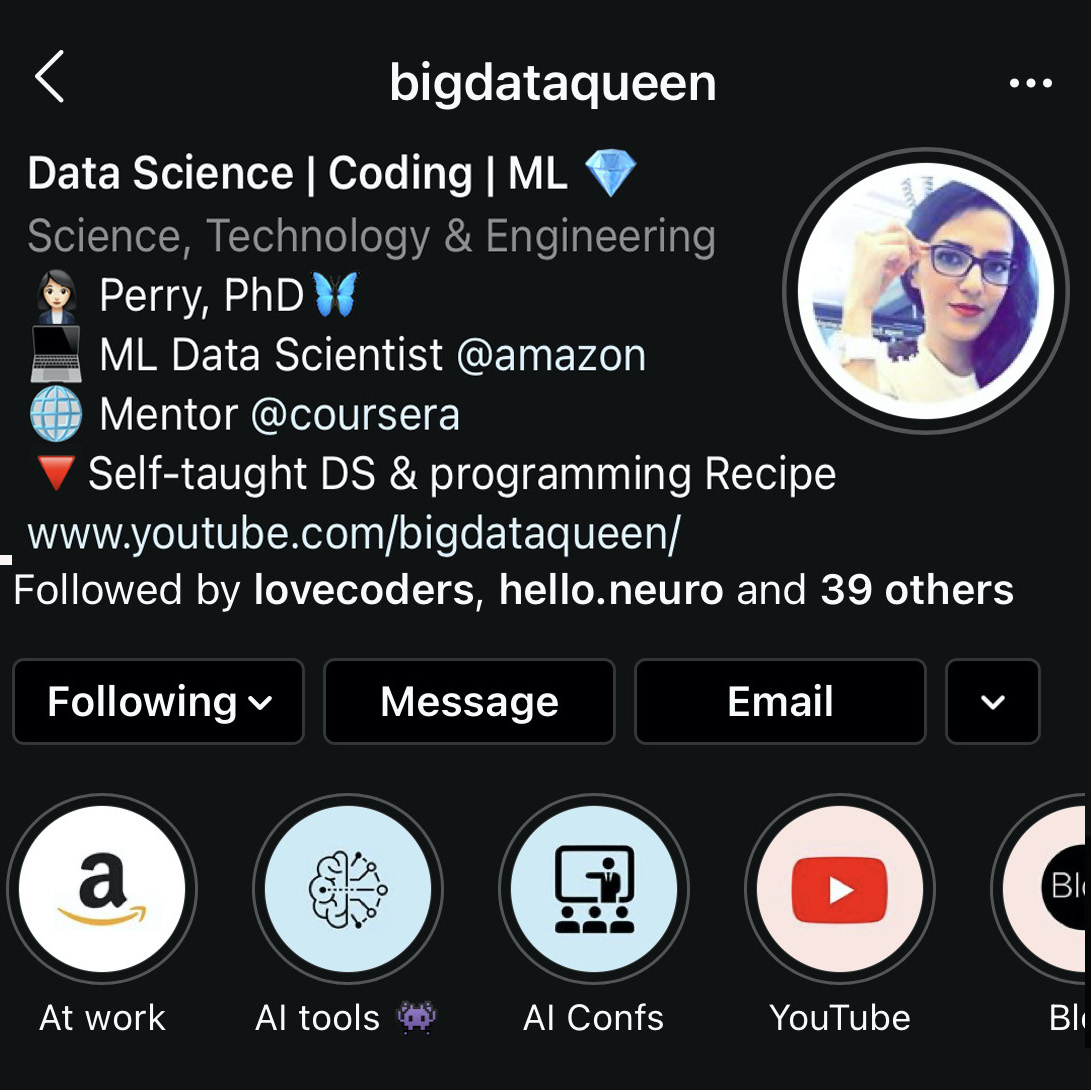
\includegraphics[width=5cm]{instagram_example2.jpg}
%		\caption{A design concept of @bigdataqueen new public profile overview.}
%		\label{fig:instagram_new_overview}
%	\end{center}
%\end{figure}

	


\section{Write up your results}

	Section intro.

	\begin{table}[ht]
		\centering
		\begin{tabular}[t]{|c| c |}
			\hline
			Gener & Total  \\ 
			\hline
			Male & 7 \\ 
			\hline
			Female & 9  \\ 
			\hline
			Prefer not to say &  0\\
			\hline
		\end{tabular}
		% Or to place a caption below a table
		\caption{The total number of participants by gender.}
		\label{tab:gender}
	\end{table}%


	After conducting the questionnaire, we had a total of 16 responses. Seven responses were male participants, and nine were female (see table: \ref{tab:gender}). While it is not exactly fifty-fifty in terms of male and female participants, it is fairly close in terms of their being less likely for any bias within the results and giving a good generalisation. 
	
	\begin{table}[ht]
		\centering
		\begin{tabular}[t]{ |c| c | }
			\hline
			In what direction would you say & \\
			your work life balance leans towards? & Total  \\ 
			\hline
			More towards work & 5 \\ 
			\hline
			More towards life & 1  \\ 
			\hline
			Fairly equal &  10 \\
			\hline
		\end{tabular}
		% Or to place a caption below a table
		\caption{???.}
		\label{tab:work_life_swing}
	\end{table}%
	
	From the questionnaire, ten participants said that their work-life balance (see table: \ref{tab:work_life_swing}) is relatively equal, but five said they lean more towards focusing on work. What we believe is worrying is that only one participant said that they lean more towards life. So these factors bring about, do we live to work or work to live and is it the technology that is making us lean more towards work with being so easily contactable. This statement is due to (see table: \ref{tab:app_impact}) the question of "what applications have the biggest impact (positive and/or negative) on your work-life balance" and IM receiving fourteen votes. So that means that only two participants feel that their IM does not impact on their work-life balance. While ten participants have said emails impact them. However, when we look at the average scores of the individual apps and devices impact (see table: \ref{tab:general_qs}), we can see that mobile phones and IM both had an average score of 3.5. Therefore meaning the results were leaning more towards having a negative impact. While on the other hand, emails were 3.1, so learning towards a more neutral impact but yet email was the second most significant impact on work-life balance. So could this mean that people think emails impact them more than they do and that IM is the main application that impacts that balance?




When we look at the results in table \ref{tab:device_social}, we can see that 100\% of the participants said that the mobile phone was the device they used the most when doing personal tasks. However, when we look at the impact of mobile phones, the average score is 3.5. Showing that the mobile phone generally has a more negative impact, but if it is the phone is what they use for the user's life tasks, is it that the phone is harming work or their private life? 

\begin{table}[ht]
	\centering
	\begin{tabular}[t]{ |c| c | }
		\hline
		What Applications have the biggest & \\
		impact (positive and/or negative) & \\
		on your work-life balance?  & Total  \\ 
		\hline
		Emails & 10 \\ 
		\hline
		Mindfull Apps & 6  \\ 
		\hline
		Instand Messaging &  14 \\
		\hline
		
	\end{tabular}
	% Or to place a caption below a table
	\caption{????.}
	\label{tab:app_impact}
\end{table}%

\begin{table}[ht]
	\centering
	\begin{tabular}[t]{ |c| c | }
		\hline
		What device have the biggest & \\
		impact (positive and/or negative) & \\
		on your work-life balance?  & Total  \\ 
		\hline
		Desktop Computer & 0 \\ 
		\hline
		Laptop & 3  \\ 
		\hline
		Mobile Device &  13 \\
		\hline
		
	\end{tabular}
	% Or to place a caption below a table
	\caption{????.}
	\label{tab:device_impact}
\end{table}%

\begin{table}[ht]
	\centering
	\begin{tabular}[t]{ |c| c | }
		\hline
		What device do you use the most for work? & Total  \\ 
		\hline
		Desktop Computer & 6 \\ 
		\hline
		Laptop & 9  \\ 
		\hline
		Mobile Device &  1 \\
		\hline
	\end{tabular}
	% Or to place a caption below a table
	\caption{????.}
	\label{tab:device_work}
\end{table}%
	

\begin{table}[ht]
	\centering
	\begin{tabular}[t]{ |c| c | }
		\hline
		What device do you use the most for social? & Total  \\ 
		\hline
		Desktop Computer & 0 \\ 
		\hline
		Laptop & 0  \\ 
		\hline
		Mobile Device &  16 \\
		\hline
	\end{tabular}
	% Or to place a caption below a table
	\caption{????.}
	\label{tab:device_social}
\end{table}%

\begin{table}[ht]
	\centering
	\begin{tabular}[t]{ |c| c | }
		\hline
		Question & Average Result  \\ 
		\hline
		How important is work & \\
		life balance to you? & \\
		1: Not Important & \\
		5: Very Important & 4.8 \\ 
		\hline
		How much would you say & \\
		emails impacts on your & \\
		work-life balance? & \\
		1: Improves Balance & \\
		5: Negative Effect & 3.1  \\ 
		\hline
		How much would you say & \\
		Instant messaging impacts on your & \\
		work-life balance? & \\
		1: Improves Balance & \\
		5: Negative Effect & 3.5 \\
		\hline
		How much would you say & \\
		mindful apps impacts on your & \\
		work-life balance? & \\
		1: Improves Balance & \\
		5: Negative Effect & 2.8 \\
		\hline
		How much would you say & \\
		mobile devices impacts on your & \\
		work-life balance? & \\
		1: Improves Balance & \\
		5: Negative Effect & 3.5 \\
		\hline
	\end{tabular}
	% Or to place a caption below a table
	\caption{????.}
	\label{tab:general_qs}
\end{table}%	


\section{Conclusion}
	 
	one one one one one one one one one one one one one one one one one one one one one one one one one one one one one one one one one one one one one one one one one one one one one one one one one one one one one one one one one one one one one one one one one one one one one one one one one one one one one one one one one one one one one one one one one one one one one one one one one one one one one one one one one one one one one one one one one one one one one one one one one one one one one one one one one one one one one one one one one one one one one one one one one one one one one one 
	
% BALANCE COLUMNS
\balance{}

% REFERENCES FORMAT
% References must be the same font size as other body text.
\bibliographystyle{SIGCHI-Reference-Format}
\bibliography{sample}

\end{document}

%%% Local Variables:
%%% mode: latex
%%% TeX-master: t
%%% End:
